\chapter{Experimental Results}

All experiments in this thesis used a set of standard conditions.  First, the length and width of each puzzle piece was set to 28~pixels per the standard established by~\cite{cho2010} and subsequently used by~\cite{pomeranz2011, gallagher2012, sholomon2013, paikin2015}. What is more, the Mixed-Bag Solver was passed no information concerning piece location nor rotation.  Furthermore, no information concerning the size of the dimensions or number of pieces in each ground-truth image is provided to the solver.  Concerning the number of input puzzles, Paikin~\& Tal's algorithm requires this information; as such, all runs of their algorithm were supplied this, meaning their algorithm is by definition solving a simpler problem.  Despite that, the Mixed-Bag Solver still generally outperforms their algorithm.

\section{Accuracy Determining the Number of Input Puzzles}

For the Mixed-Bag Solver to provide meaningful outputs, it must be able to identify the number of ground-truth inputs provided to the solver.  The test dataset used to measure the solver's performance in this area was published by Pomeranz~\textit{et al.} in~\cite{pomeranzBenchmarkImages}; the dataset consists of 20~images, each of which has 805~pieces.

The next subsection discusses the solver's performance when provided only a single image.  This is separated from the more general discussion as the algorithm's performance on a single image marks the ceiling of its performance.  The algorithm's performance when solving two to five puzzles is discussed in a separate subsection.

\subsection{Single Puzzle Solving}

The Mixed-Bag solver was able to correctly identify the single ground-truth image for  17~out of the 20~images (i.e., 85\% accuracy).  For the remaining 3~images, the solver estimated that there were 2~images, meaning the error was at most only a single puzzle.  Appendix~\ref{chap:incorreclyClassifiedSingleImages} shows the ground-truth image as well as the outputs from Paikin~\& Tal's algorithm as well as this thesis' Mixed-Bag Solver.  

The Mixed-Bag Solver struggled to correctly identify the number of inputs when the image has large areas with little variation (e.g., a blue sky, smooth water, etc.). Two example images from the test dataset are shown in Figure~\ref{fig:pomeranzBestBuddiesVisualizations} shows two images in the Pomeranz~\textit{et al.}.  The Mixed-Bag Solver was able to perfectly reconstruct image~(a); in contrast, the Mixed-Bag Solver thought the pieces from image~(b) came from two separate puzzles.\footnote{Appendix~\ref{chap:incorreclyClassifiedSingleImages} shows the three images that were incorrectly identified by the Mixed-Bag Solver as well as the solver outputs generated.} The best buddy visualizations in Figure~\ref{fig:pomeranzBestBuddiesVisualizations} shows two images in the Pomeranz~\textit{et al.} show that image~(a) had a significantly higher best buddy density as well as much fewer interior non-adjacent best buddies.  It is these two factors the contributed the most to the Mixed-Bag Solver being unable to determine the number of input images for the three puzzles. 

\begin{figure}[tb]
\centering
  \begin{tabular}{ >{\centering\arraybackslash}m{0.47\textwidth} >{\centering\arraybackslash}m{0.47\textwidth} }

	\fbox{\includegraphics[scale=0.18]{./images/single_puzzle/pomeranz_805_14.jpg}} & \fbox{\includegraphics[scale=0.18]{./images/single_puzzle/best_buddies_pomeranz_805_14.jpg}} \\~\\
	Ground-Truth Image~(a) & Best Buddy Visualization of Image~(a) 
\\~\\
	\fbox{\includegraphics[scale=0.18]{./images/single_puzzle/pomeranz_805_12.jpg}} & \fbox{\includegraphics[scale=0.18]{./images/single_puzzle/best_buddies_pomeranz_805_12.jpg}} \\~\\
	Ground-Truth Image~(b) & Best Buddy Visualization of Image~(b) 
  \end{tabular}
\caption{Comparison of Best Buddy Density and Interior Non-Adjacent Best Buddies for Two Images from the Pomeranz \textit{et al.} 805 Piece Dataset}
\label{fig:pomeranzBestBuddiesVisualizations}
\end{figure} 

It is important to note that the difficulty the Mixed-Bag Solver has reconstructing images with low Best Buddy Density is actually an artifact of the assembler and not the solver.  Paikin~\& Tal mentioned in~\cite{paikin2015} that their solver may yield ``unsatisfactory results'' on such images.

\subsection{Multiple Puzzle Solving}

When testing the ability of the Mixed-Bag Solver to accurately determine the number of input puzzles, images were randomly selected from the 805~piece, 20~image dataset, without replacement.  In total, Table~\ref{tab:numberSolverIterations} shows the number of times the solver was run for each input size.  As explained in Section~\ref{sec:assemblerTimeComplexity}, Paikin~\& Tal's solver can execution time can grow cubicly, in particular if Best Buddy Density is low.  As such, the solver was performed few times as the new number of input puzzles increased.

\begin{table}[tb]
\begin{center}
\begin{tabular}{ c||c|c|c|c } 
 \toprule
 \# Puzzles    &  2 &  3 & 4 & 5 \\ 
\hline \hline
 \# Iterations & 55 & 25 & 8 & 5 \\ 
 \bottomrule
\end{tabular}
\end{center}
\caption{Number of Solver Iterations for Each Puzzle Input Count}\label{tab:numberSolverIterations}
\end{table}

Figure~\ref{fig:inputPuzzleCountErrorFrequency} shows the frequency with which the Mixed-Bag Solver estimated the number of input puzzles.  A correct estimation of the number of puzzles would represent an error of ``0.''  An over estimate of a single puzzle (e.g., identifying four puzzles when only three were input to the solver) would represent an error of ``1.''  Across all of the experiments, the Mixed-Bag Solver never under estimated the number of input puzzles.  

\begin{figure}
\begin{center}
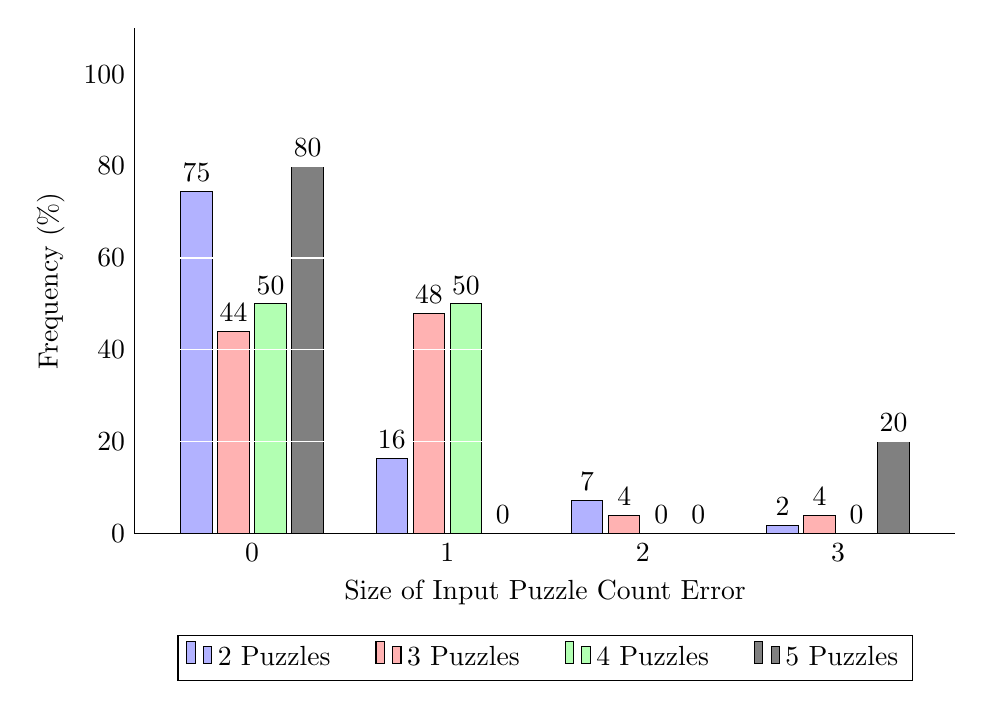
\begin{tikzpicture}
  \begin{axis}[
        ybar, axis on top,
        height=8cm, width=12cm,
        bar width=0.4cm,
        ymajorgrids, tick align=inside,
        major grid style={draw=white},
        enlarge y limits={value=.1,upper},
        ymin=0, ymax=100,
        axis x line*=bottom,
        axis y line*=left,
        y axis line style={opacity=1},
        tickwidth=0pt,
        enlarge x limits=0.2,
        legend style={
            at={(0.5,-0.2)},
            anchor=north,
            legend columns=-1,
            /tikz/every even column/.append style={column sep=0.5cm}
        },
        xlabel={Size of Input Puzzle Count Error},
        ylabel={Frequency (\%)},
        symbolic x coords={
           0, 1, 2, 3},
       xtick=data,
       nodes near coords={
        \pgfmathprintnumber[precision=0]{\pgfplotspointmeta}
       }
    ]
\addplot [fill=blue!30]
	coordinates {(0,74.5) (1,16.4)
		 (2,7.3) (3,1.8)};
\addplot [fill=red!30]
	coordinates {(0,44) (1,48)
		 (2,4) (3,4)};
\addplot [fill=green!30]
	coordinates {(0,50) (1,50)
		 (2,0) (3,0)};
\addplot 
	coordinates {(0,80) (1,0)
		 (2,0) (3,20)};
\legend{2 Puzzles, 3 Puzzles, 4 Puzzles, 5 Puzzles}
\end{axis}
\end{tikzpicture}
\end{center}
\caption{Mixed-Bag Solver's Input Puzzle Count Error Frequency}
\label{fig:inputPuzzleCountErrorFrequency}
\end{figure}

In this set of experiments, the Mixed-Bag solver correctly determined the number of input puzzles in 65\% of the tests.  Likewise, in less than 8\% of the tests did the solver over-estimate the number of input puzzles by more than one.  Since the solver never underestimated the number of input puzzles, it is expected that the performance of the solver would be improved by reducing the minimum clustering threshold discussed in Section~\ref{sec:hierarchicalClustering}. 

\section{Ten Puzzle Solving}

Paikin~\& Tal's~\cite{paikin2015} algorithm was shown to be able to solve up to five images simultaneously, which represents the most in the current literature.  To achieve this, their solver needed to be supplied with the number of input puzzles.  In contrast, this Mixed-Bag Solver has been shown to be able to solve up to ten puzzles of varying size.  Appendix~\ref{chap:tenPuzzleSolving} shows the input puzzles as well as the Mixed-Bag Solver's outputs. When the identical set of puzzles were supplied to Paikin~\& Tal's algorithm, the seeds for nine of the puzzles came from just three of the input puzzles.  

Table~\ref{tab:pomeranzBestBuddiesVisualizations} shows a comparison of the results between this thesis' Mixed-Bag Solver (MBS) and Paikin~\& Tal's algorithm's.  Despite the Mixed-Bag Solver receiving less information, it significantly outperformed Paikin~\& Tal receiving greater than 90\% accuracy for both  Shiftable Enhanced Direct Accuracy Score (SEDAS), and the Enhanced Neighbor Accuracy Score (ENAS) on all puzzles.  In contrast, Paikin~\& Tal only exceeded 90\% SEDAS and ENAS for image~(f). 

With respect to the unshifted, Enhanced Direct Accuracy Score (EDAS) metric, only four of the Mixed-Bag's solver outputs showed a shift that would affect EDAS while 7 of Paikin~\& Tal's outputs were shifted. This indicates that the Mixed-Bag Solver has a much greater immunity to shifts than Paikin~\& Tal's algorithm.

\begin{table}[tb]
\begin{center}
\begin{tabular}{ c|c||c|c||c|c||c|c } 
 \toprule
 \multicolumn{2}{c||}{Image} & \multicolumn{2}{c||}{Shifted} & \multicolumn{2}{c||}{SEDAS} & \multicolumn{2}{c}{ENAS} \\
\hline
 ID  & \# Pieces & MBS & Paikin & MBS & Paikin & MBS & Paikin  \\ 
\hline \hline
 (a) &  264     & No  & Yes & 100\%  & 0\% & 100\% & 54.4\% \\ 
\hline
 (b) &  330     & No  & Yes & 100\%  & 0\% & 100\% &  9.0\% \\ 
\hline
 (c) &  432     & Yes & Yes & 90.5\% &  0\%   & 91.1\% & 3.4\% \\  
\hline
 (d) &  540     & No  & No  & 97.8\% & 52.6\% & 97.5\% & 50.9\% \\ 
\hline
 (e) &  540     & No  & No  & 100\%  &  5.9\% & 100\%  & 32.7\% \\ 
\hline
 (f) &  540     & Yes & No  & 97.8\% & 94.3\% & 91.7\% & 93.1\% \\ 
\hline
 (g) &  805     & No  & Yes & 99.7\% &  0\%   & 99.0\% &  7.7\% \\ 
\hline
 (h) &  805     & Yes & Yes & 95.8\% &  0\%   & 96.7\% &  7.0\% \\ 
\hline
 (i) &  805     & No  & Yes & 100\%  &  0\%   & 100\%  &  31.1\% \\ 
\hline
 (j) &  805     & Yes & Yes & 99.8\% &  0\%   & 99.0\% &   7.3\% \\ 
 \bottomrule
\end{tabular}
\end{center}
\caption{Comparison of the SEDAS, EDAS, and ENAS Results for the 10 Puzzle Dataset}\label{tab:pomeranzBestBuddiesVisualizations}
\end{table}